\documentclass[11pt]{article}
\usepackage[T1]{fontenc}
\usepackage[utf8]{inputenc}
\usepackage[
    left=1in,
    right=1in,
    top=0.6in,
    bottom=1in
]{geometry}

\usepackage{amsmath,amssymb}
\usepackage{graphicx}
\usepackage{booktabs}
\usepackage{float}
\usepackage[hidelinks]{hyperref}
\usepackage{tabularx}
\usepackage{tikz}
\usetikzlibrary{arrows.meta,positioning}

\title{Force Feedback Refinement}
\author{ARC Students}
\date{\today}

\begin{document}
\maketitle

%==============================================================================
\section{Defining the Problem}

\begin{center}
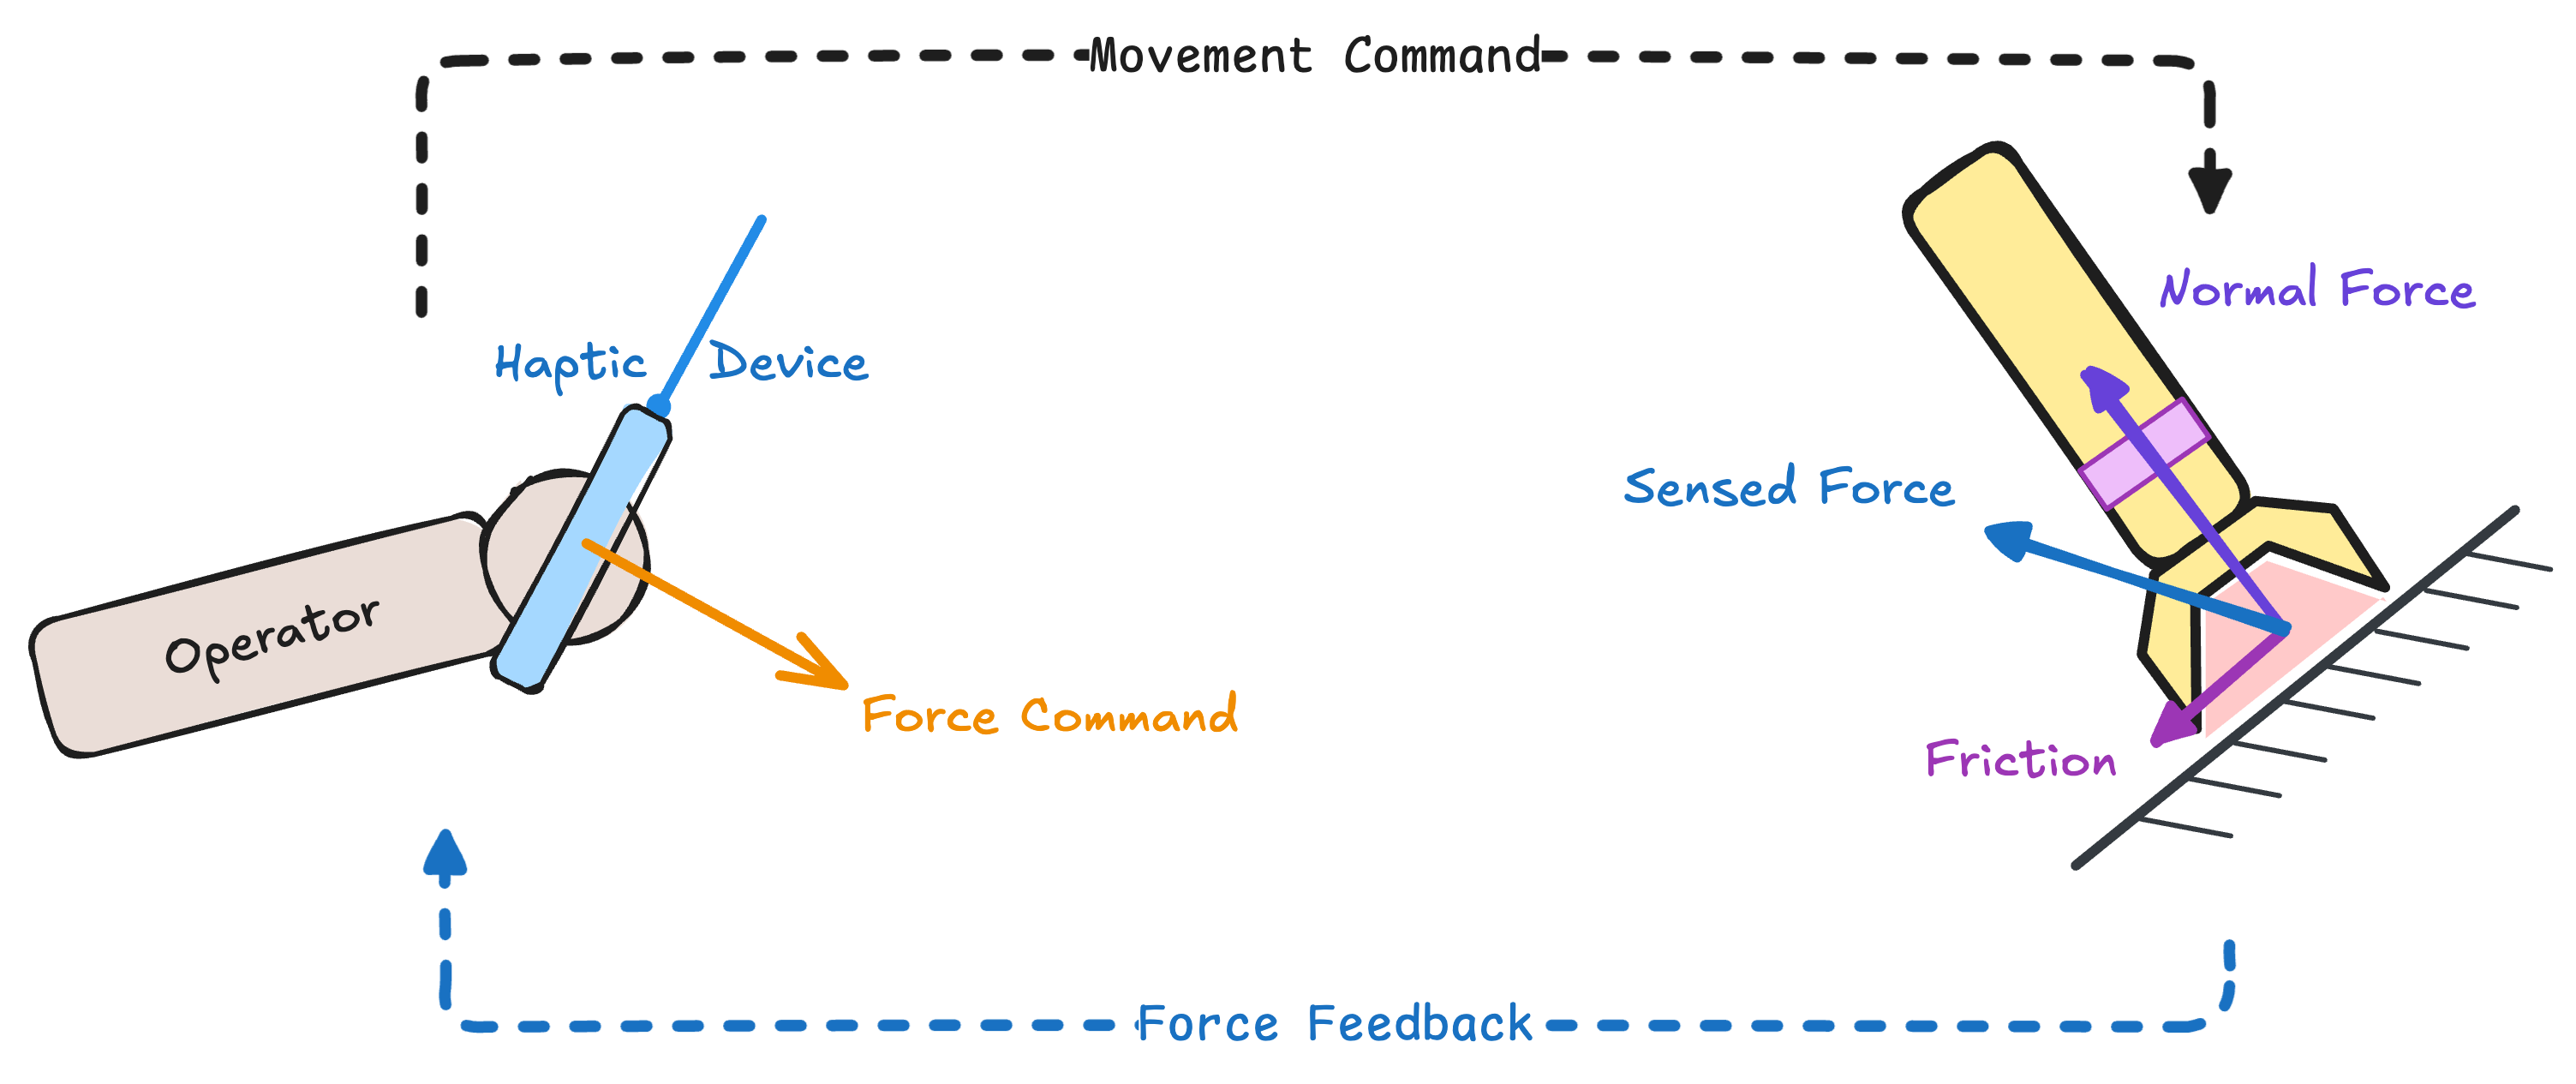
\includegraphics[width=0.9\textwidth]{drawings/ForceFeedback.png}
\end{center}

During tele-op, the end effector tracks the position the operator specifies via a controller. Our problem is: how to meaningfully reflect the measured force to the operator?

We define the action space in a 3D world; every vector and matrix below has:
\begin{equation*}
\vec{v} \in \mathbb{R}^3 \quad\quad [A]\in\mathbb{R}^{3\times3}
\end{equation*}
We only consider translational force feedback; torque is similar.

\subsection{Controller Space and Robot Space}

The controller polls the current position of the pen $\vec{p}$ in the controller space; we map it to the reference point in robot space through a linear function. The function is reversible.
\begin{equation*}
M(\vec{p})=s[R]\vec{p} + \vec{r}_0 = \vec{r} \quad\quad M^{-1}(\vec{r})=\vec{p}
\end{equation*}
where $s$ is the scaling factor, $[R]$ is the rotation from controller space to robot space, and $\vec{r}_0$ is the zero-reference. In real life, it gets reset every time the operator picks up control again. Here, since the pilot remains in control, we treat it as a constant.

Let the actual (measured) state of the robot be:
\begin{equation*}
\{\, \text{Position: } \,\vec{x} \quad\quad \text{Velocity: } \,\dot{\vec{x}} \quad\quad \text{Acceleration: } \,\ddot{\vec{x}} \,\}
\end{equation*}

\subsection{Applied and Measured Force}

The operator's hand applies a force $\vec{F}_o$ to the Haply controller.
The controller renders the feedback force $\vec{F}_b$ back onto the operator's hand.
\begin{equation*}
\vec{F}_o = - \vec{F}_b
\end{equation*}

On the robot side, we measure the raw force $\vec{F}_s$, and denote its filtered version as $\vec{F}_s^\ast$.
The raw reading is not yet the contact force $\vec{F}_c$ that the environment exerts on the end-effector: it also includes the inertia and weight of the end-effector, which has mass $m$:
\begin{equation*}
\vec{F}_s = \vec{F}_c - m\ddot{\vec{x}} - mg\,\hat{k}
\end{equation*}
Here $g$ is the gravitational acceleration and $\hat{k}$ is the upward unit vector.

Let $\hat{n}$ be the direction of the end-effector head.
The contact force splits into the normal force $\vec{F}_n$ along $\hat{n}$, and the friction $\vec{f}$ perpendicular to it:
\begin{equation*}
\vec{F}_n = \text{proj}_{\hat{n}}\,\vec{F}_c \quad\quad \vec{f} = \vec{F}_c - \vec{F}_n
\end{equation*}

%==============================================================================
\section{Baseline Method}

The baseline feeds back a blend of two $z$-axis forces, scaled by the gain $\lambda$:
\begin{equation*}
F_{b,z} = \lambda\,\big[(1-\alpha)\,F^\ast_{s,z} + \alpha\,F_{\text{wall},z}\big]
\end{equation*}
\begin{itemize}
    \item \textbf{Direct force feedback:} the filtered force $F^\ast_{s,z}$.
    \item \textbf{Virtual wall with deadzone:} once $F_{s,z}$ exceeds a threshold, a wall is fixed at $p_\text{wall} = p_z + F^\ast_{s,z}/K$ and pushes back with $F_{\text{wall},z} = K\,(p_\text{wall} - p_z) - B\,\dot{p}_z$; below the threshold, $\alpha = 0$.
\end{itemize}

%==============================================================================
\section{Admittance Controller}

\subsection{Purpose}

We want to control the amount of force applied on the object by the end-effector.

However, we can’t control force precisely: motor torque control is open-loop; UR robots don’t support it anyways. We only have a strong position controller that rigorously follows the reference, even when that means smashing hard into obstacles.

\subsection{Modeling}

The solution is to simulate a classic \textbf{impedance control model}. The operator holds the tool from a spring of \emph{negligible length}.
\begin{itemize}
    \item The hand represents reference pose $\vec{r}$, the tool represents end-effector position $\vec{x}$, the spring has impedance $K_p$.
    \item The spring has some damping factor too.
    \item The object exerts a force $\vec{F}_\text{ext}$ to the tool, and we wish to apply an additional $\vec{F}_\text{ref}$ onto the object.
\end{itemize}

\begin{center}
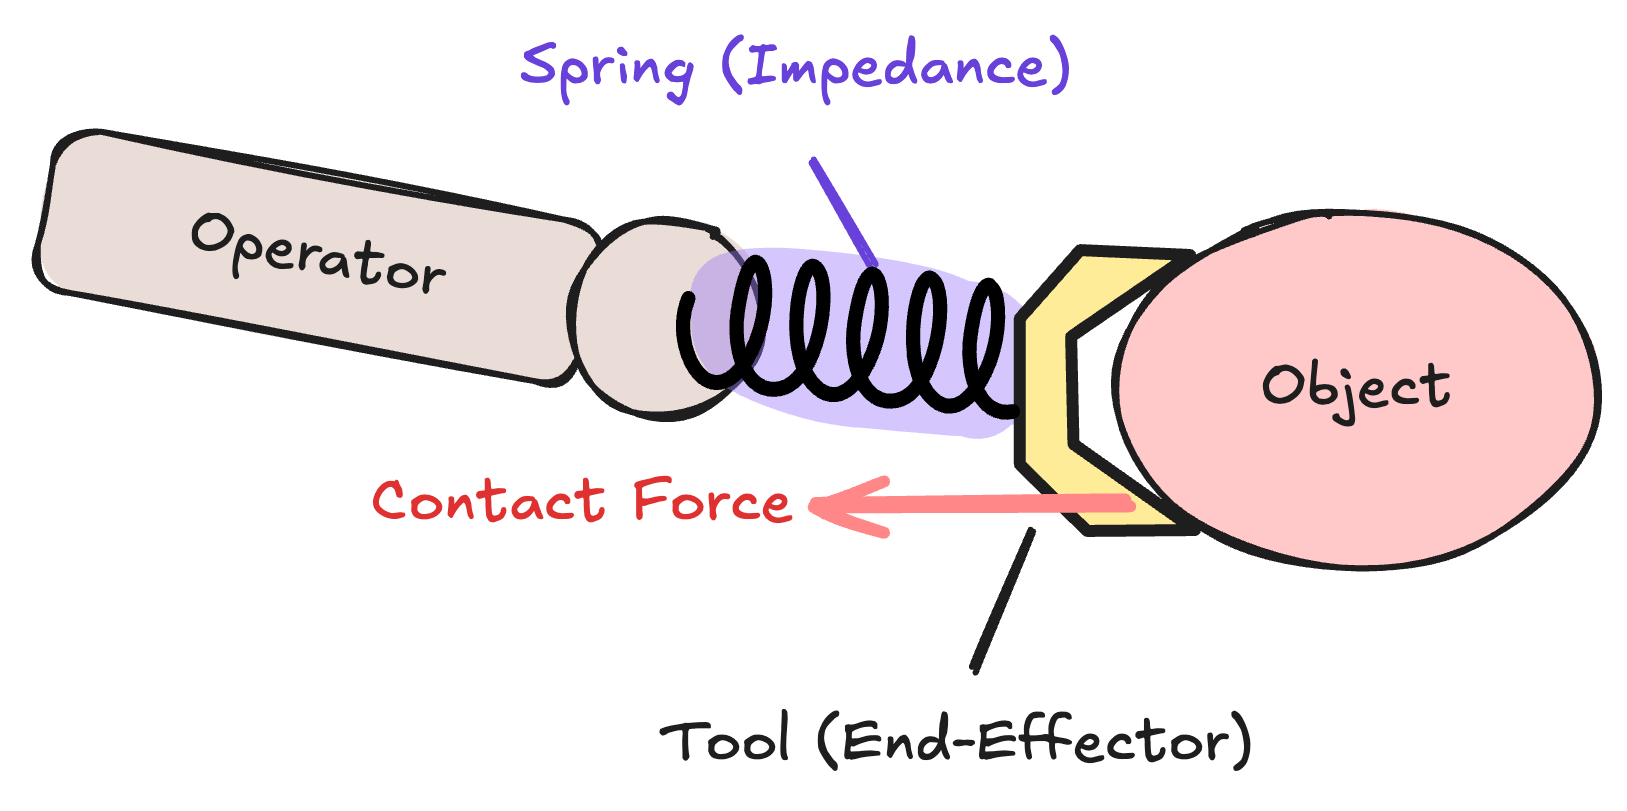
\includegraphics[width=0.6\textwidth]{drawings/Impedance Model.png}
\end{center}

We can write a differential equation:
\begin{equation*}
m_\text{vir} \,\ddot{\vec{x}} = \underbrace{K_p (\vec{r}-\vec{x})}_{\text{Impedance}} \,-\, \underbrace{K_d \dot{\vec{x}}}_{\text{Damping}} \,+\, \underbrace{(f_\text{ext} + f_\text{ref})^{*}}_{\text{Force Term}}
\end{equation*}

And we send the result of this simulation to the rigorous position controller instead.

\subsection{Feedback}

Now we ask in this model what the force that the tool feeds back to the operator? It turns out to be exactly equal to the force of the spring. This can be written as a simple PD controller.
\begin{equation*}
\vec{F}_b = K_p(\vec{x}-\vec{r}) - K_d \,\dot{\vec{r}}
\end{equation*}

%==============================================================================
\section{Async Feedback System}

In the baseline system, everything is synchronous, and we have to trade filtering quality for reactiveness.

Here, the force model can be sent from the robot at a lower frequency as an impedance model, leaving time for fine filtering. The high-frequency force feedback loop gives instant responses to operator inputs.

\begin{center}
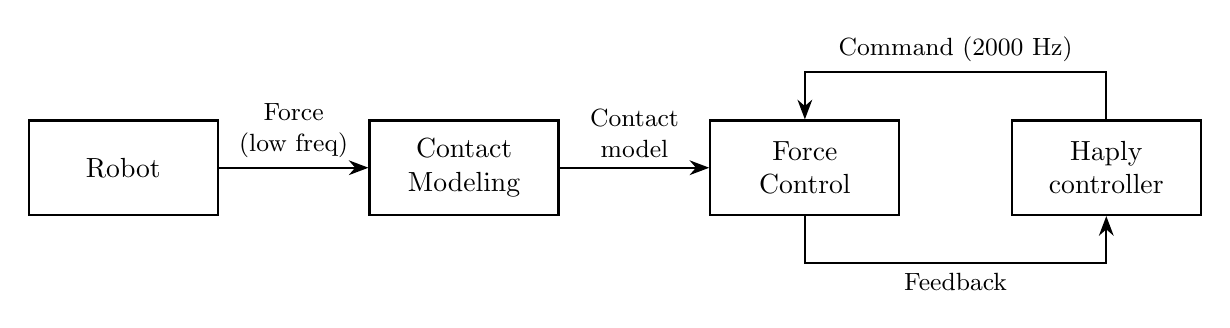
\begin{tikzpicture}[
    box/.style={draw, thick, minimum width=2.4cm, minimum height=1.2cm, align=center},
    lbl/.style={font=\small, align=center},
    >={Stealth[length=2.5mm]}
]
    \node[box] (R) {Robot};
    \node[box, right=1.9cm of R] (CM) {Contact\\Modeling};
    \node[box, right=1.9cm of CM] (FC) {Force\\Control};
    \node[box, right=1.4cm of FC] (H) {Haply\\controller};
    \draw[->, thick] (R) -- node[lbl, above] {Force\\(low freq)} (CM);
    \draw[->, thick] (CM) -- node[lbl, above] {Contact\\model} (FC);
    \draw[->, thick] (H.north) -- ++(0,0.6) -| node[lbl, pos=0.25, above] {Command (2000 Hz)} (FC.north);
    \draw[->, thick] (FC.south) -- ++(0,-0.6) -| node[lbl, pos=0.25, below] {Feedback} (H.south);
\end{tikzpicture}
\end{center}

%==============================================================================
\section{Sensor Calibration}

To isolate the contact force $\vec{F}_c$, we need to estimate $m$ and $g$.
The sensor cannot be zeroed, so we apply linear system identification instead.

\subsection{Tilting the Arm}

\begin{center}
\begin{minipage}[c]{0.38\textwidth}
    \centering
    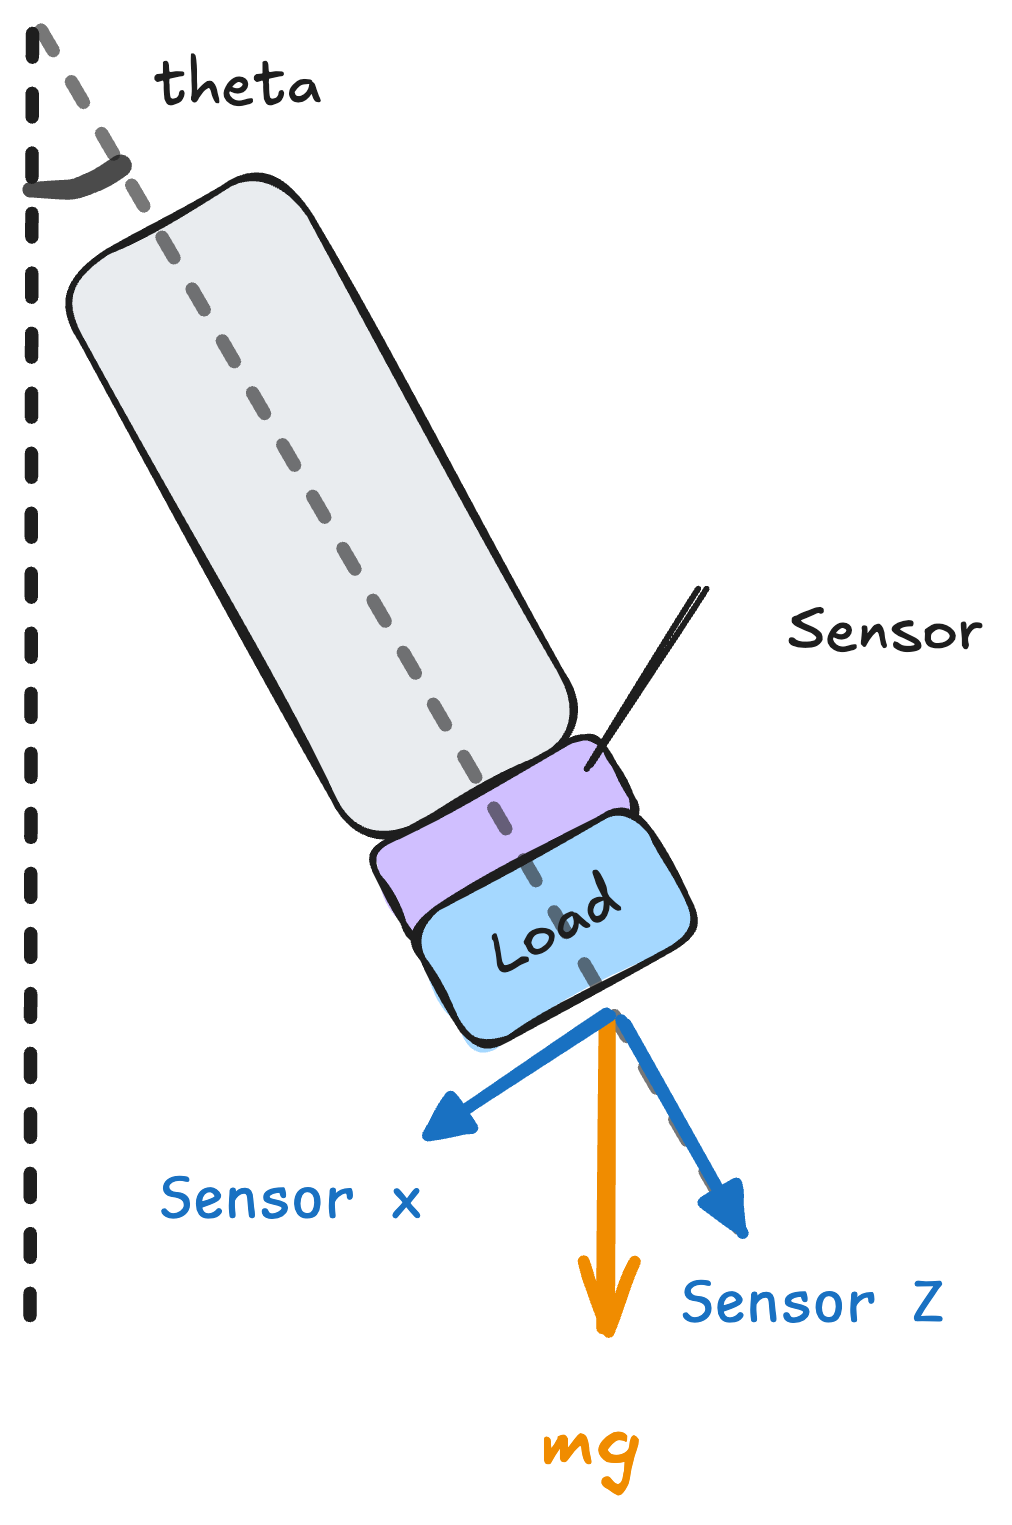
\includegraphics[width=\linewidth]{drawings/SystemID_1.png}
\end{minipage}\hfill
\begin{minipage}[c]{0.38\textwidth}
    \centering
    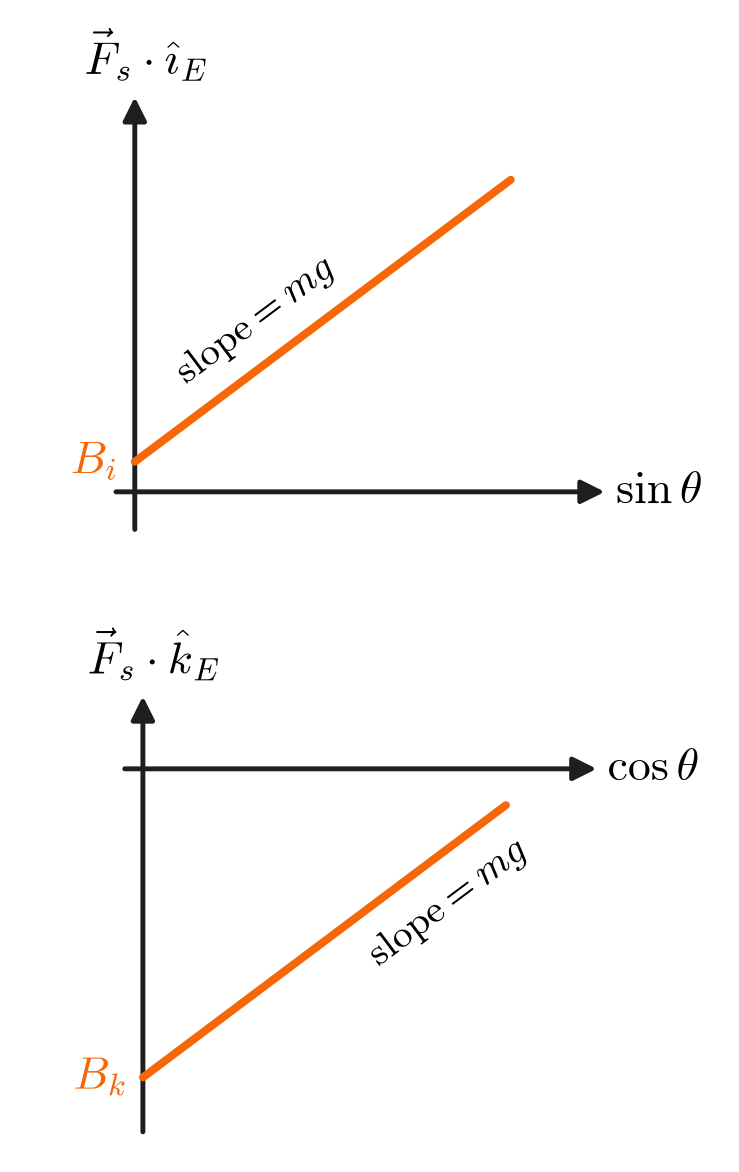
\includegraphics[width=\linewidth]{media/sysid-tilt-plots.png}
\end{minipage}
\end{center}

With the load hanging below the sensor, rotate the arm upwards so that the head direction $\hat{n}$ tilts by $\theta$ from the vertical.
In the end-effector frame $(\hat{i}_E, \hat{k}_E)$, the sensor reads:
\begin{equation*}
\begin{cases}
\vec{F}_s \cdot \hat{k}_E = mg\cos\theta + B_k \\
\vec{F}_s \cdot \hat{i}_E = mg\sin\theta + B_i
\end{cases}
\end{equation*}
Plot each component against $\cos\theta$ and $\sin\theta$: the slope yields the value of $mg$, and the intercepts give the biases $B_k$ and $B_i$.

\subsection{Spiral Trajectory}

\begin{center}
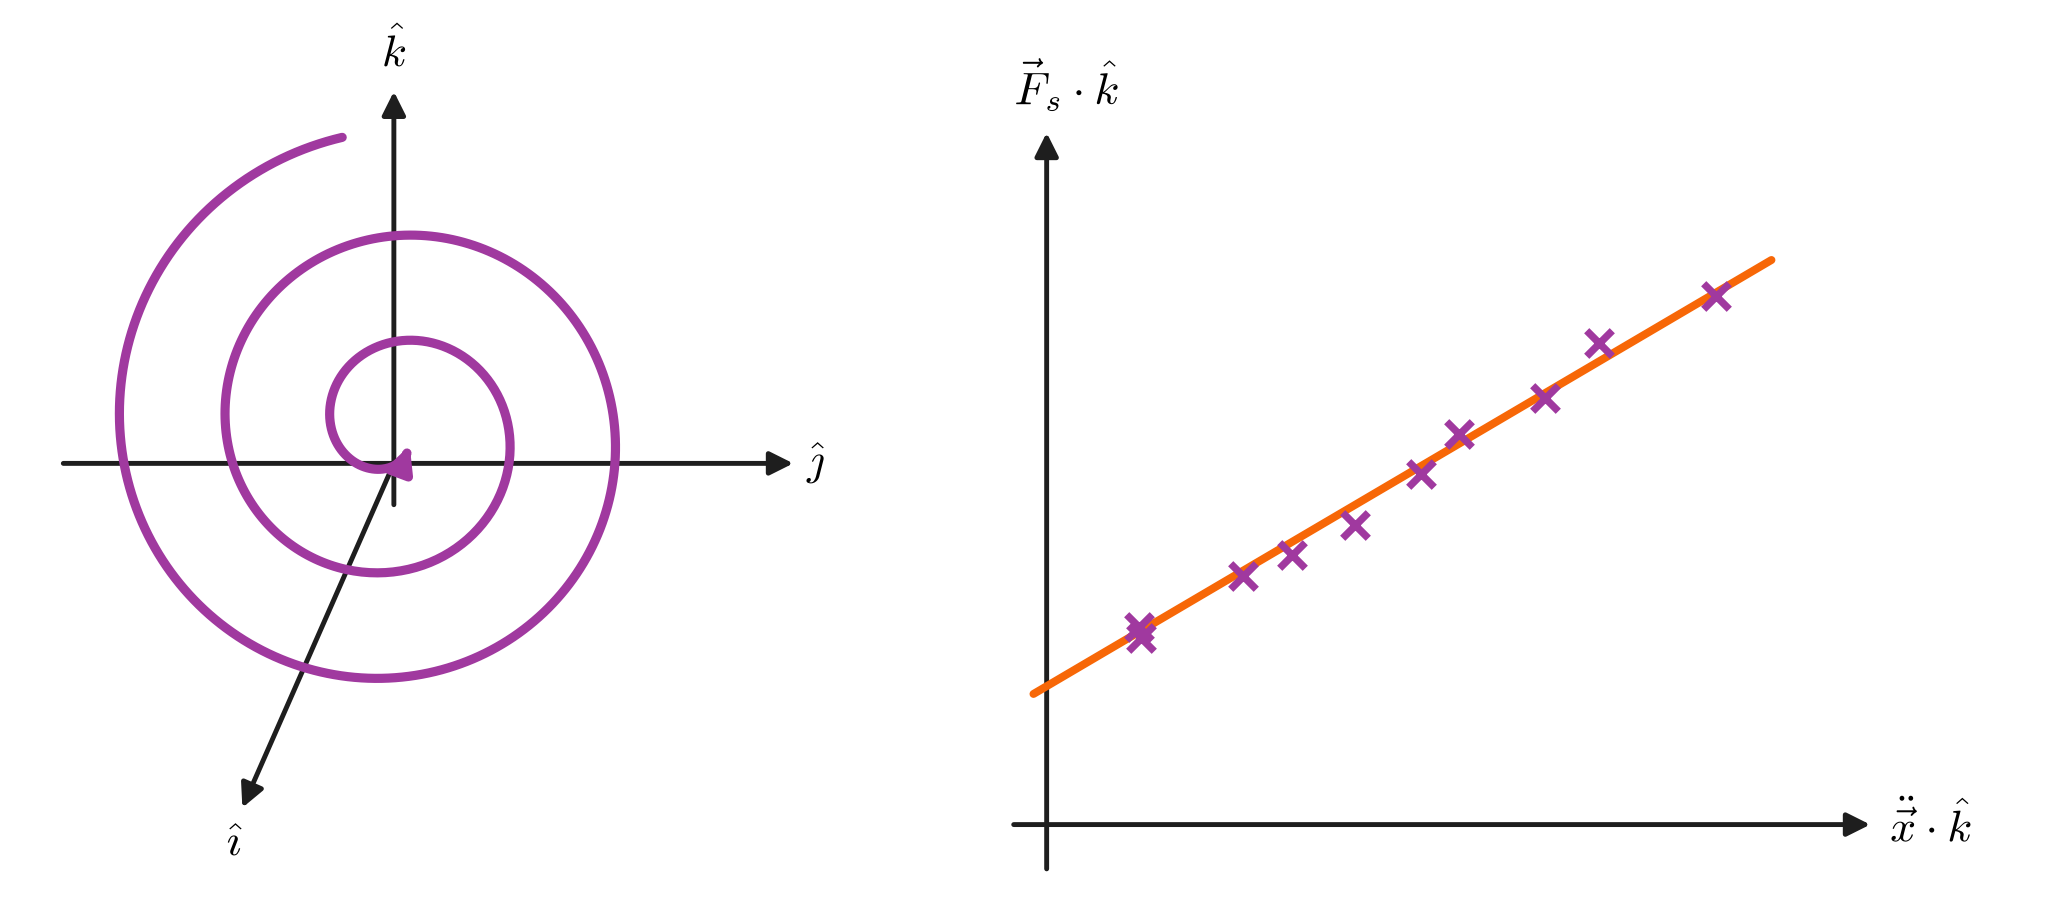
\includegraphics[width=0.72\textwidth]{media/sysid-spiral.png}
\end{center}

Move the end-effector along a spiral in the vertical $\hat{j}$--$\hat{k}$ plane.
Plot $\vec{F}_s \cdot \hat{k}$ against $\ddot{\vec{x}} \cdot \hat{k}$, and fit a line through the samples.

\end{document}
